\documentclass{beamer}
%
% Choose how your presentation looks.
%
% For more themes, color themes and font themes, see:
% http://deic.uab.es/~iblanes/beamer_gallery/index_by_theme.html
%
\mode<presentation>
{
  \usetheme{Boadilla}      % or try Darmstadt, Madrid, Warsaw, ...
  \usecolortheme{beaver} % or try albatross, beaver, crane, ...
  \usefonttheme{default}  % or try serif, structurebold, ...
  \setbeamertemplate{navigation symbols}{}
  \setbeamertemplate{caption}[numbered]
  
} 

\usepackage{xcolor,colortbl}
\usepackage[english]{babel}
\usepackage[utf8x]{inputenc}
\usepackage{courier}
\usepackage{dsfont}
\usepackage{verbatim} 
\usepackage{enumerate}
\usepackage{tikz}
\usepackage{multirow}
\usepackage{bbm}
\usepackage{amsmath}
\usepackage{venndiagram}
\usepackage{epigraph} 
%\usepackage{xcolor}

%\usepackage{enumitem}

\usepackage{hyperref}
\hypersetup{
    colorlinks=true,
    linkcolor=blue,
    filecolor=magenta,      
    urlcolor=cyan,
}

% R stuff!
\usepackage{listings}
\definecolor{codegreen}{rgb}{0,0.6,0}
\definecolor{codegray}{rgb}{0.5,0.5,0.5}
\definecolor{codepurple}{rgb}{0.58,0,0.82}
\definecolor{backcolour}{rgb}{0.95,0.95,0.92}

\lstdefinestyle{mystyle}{
    backgroundcolor=\color{backcolour},    
    commentstyle=\color{codegreen},
    keywordstyle=\color{black},
    numberstyle=\tiny\color{codegray},
    stringstyle=\color{codepurple},
    basicstyle=\ttfamily\footnotesize,
    breakatwhitespace=false,         
    breaklines=true,                 
    captionpos=b,                    
    keepspaces=true,                 
    numbers=left,                    
    numbersep=5pt,                  
    showspaces=false,                
    showstringspaces=false,
    showtabs=false,                  
    tabsize=2
}

\lstset{style=mystyle}



%% Size options for nested itemized lists
\usepackage{relsize}
\setbeamerfont{itemize/enumerate body}{parent=normal text}
\setbeamerfont{itemize/enumerate subbody}{parent=normal text,size=\relsize{-1}}
%\setbeamerfont{itemize/enumerate subsubbody}{parent=normal text,size=\relsize{-1}}




\setbeamertemplate{enumerate items}[default]
\setbeamertemplate{itemize item}[triangle]

%\setitemize{label=\usebeamerfont*{itemize item}%
%  \usebeamercolor[fg]{itemize item}
%  \usebeamertemplate{itemize item}}


\usetikzlibrary{shapes,decorations,arrows,calc,arrows.meta,fit,positioning}
\tikzset{
    -Latex,auto,node distance =1 cm and 1 cm,semithick,
    state/.style ={ellipse, draw, minimum width = 0.7 cm},
    point/.style = {circle, draw, inner sep=0.04cm,fill,node contents={}},
    bidirected/.style={Latex-Latex,dashed},
    el/.style = {inner sep=2pt, align=left, sloped}
}

\newcommand{\Mypm}{\mathbin{\tikz [x=1.4ex,y=1.4ex,line width=.1ex] \draw (0.0,0) -- (1.0,0) (0.5,0.08) -- (0.5,0.92) (0.0,0.5) -- (1.0,0.5);}}%



%% For block quote
\usepackage{etoolbox}
\AtBeginEnvironment{quote}{\par\singlespacing\small}
\newcommand{\vp}{\vspace{2mm}}

\title[Intro Statistics]{Analysis of Variance (ANOVA)}
\subtitle{}
%\author{}
\author{Grinnell College}
\date{December 2, 2024}

\graphicspath{{img/}}


\begin{document}

\begin{frame}
  \titlepage
\end{frame}

\begin{frame}{ANOVA}

Tests so far:

\begin{itemize}
\item Difference in means
\item Difference in proportion
\item Goodness of fit
\item Independence of two categorical variables
\end{itemize}

\vspace{4mm}

Today we are extending our set of tests to include testing the difference in means in multiple groups

\end{frame}


\begin{frame}{ANOVA}

The \textbf{\underline{An}alysis \underline{o}f \underline{va}riance (ANOVA)} is a collection of statistical \textit{models} used to analyze difference among many means \vspace{6mm}

The null hypothesis is testing the difference of means between $k$ groups 
\begin{align*}
H_0&: \mu_1 = \mu_2 = \dots = \mu_k \\
H_A&: \text{at least one } \mu_i \not= \mu_j
\end{align*} \vspace{4mm}

But what does this have to do with variance?
\end{frame}

\begin{frame}{Review -- Standardizing}
Think back to what we were doing when calculating test-statistics before:

\begin{align*}
T = \frac{\overline{x} - \mu_0}{(\hat{\sigma}/\sqrt{n})}
\end{align*} \vspace{4mm}

The 'formula' for a test-statistic has always been to do the following

\begin{align*}
\text{Test-stat} = \frac{\text{statistic} - \text{hypothesized value}}{\text{standard error}}
\end{align*} \vspace{2mm}

The test-statistic
\begin{itemize}
    \item measures how 'far' the statistic is from the hypothesized value
    \item uses the standard error as a 'ruler'
    \item we have been using variance to compare distance this whole time
\end{itemize}


\end{frame}


\begin{frame}{Dog Speed}
\small
Data collected by Professor Nolte: 

400 dogs from 8 different breeds (random sample of size 50 for each breed) \vspace{2mm} 

Each set has 25 black dogs and 25 dogs of one other color. For each dog, we have recorded land speeds in miles per hour (mph) \vspace{2mm}

\begin{table}[ht]
\centering
\begin{tabular}{lllr}
  \hline
Breed & Size & Other Color & N \\ 
  \hline
Chihuahua & Small & Brown & 50 \\ 
  Corgie & Small & Yellow & 50 \\ 
  Poodle & Medium & Brown & 50 \\ 
  Bulldog & Medium & White & 50 \\ 
  Saint Bernard & Large & Yellow & 50 \\ 
  German Shepard & Large & Yellow & 50 \\ 
  Mastiff & Large & Yellow & 50 \\ 
  Greyhound & Large & White & 50 \\ 
   \hline
\end{tabular}
\end{table} \vspace{2mm}

What variables will do best in helping me predict speed? Let's find out

\end{frame}


\begin{frame}{Dog Size}
\begin{center}
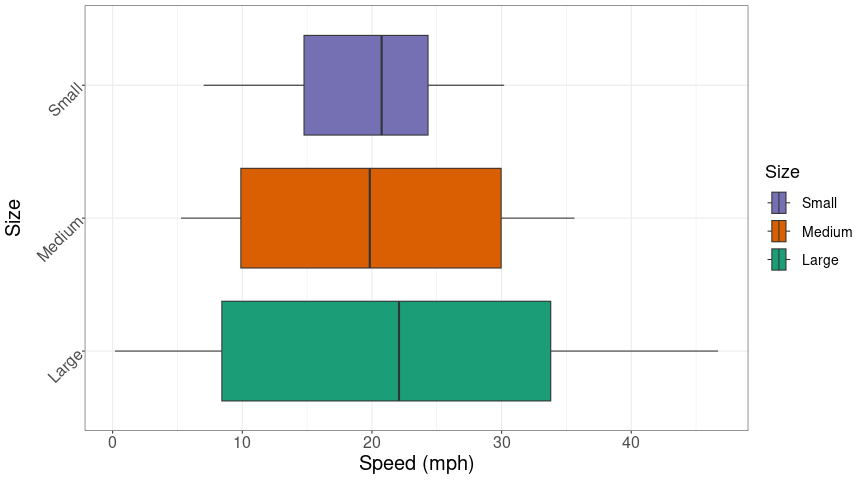
\includegraphics[scale=0.4]{img/dog_size.png}
\end{center}


\end{frame}

\begin{frame}{Dog Color}
\begin{center}
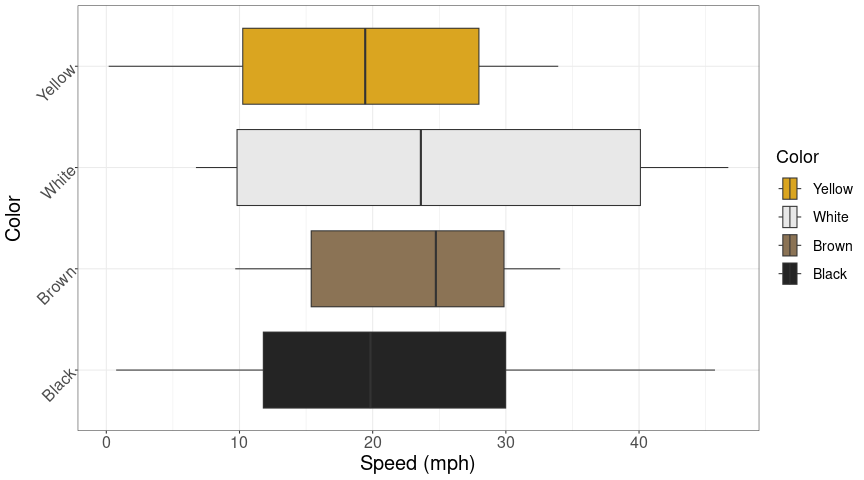
\includegraphics[scale=0.4]{img/dog_color.png}
\end{center}

\end{frame}

\begin{frame}{Dog Breed}
\begin{center}
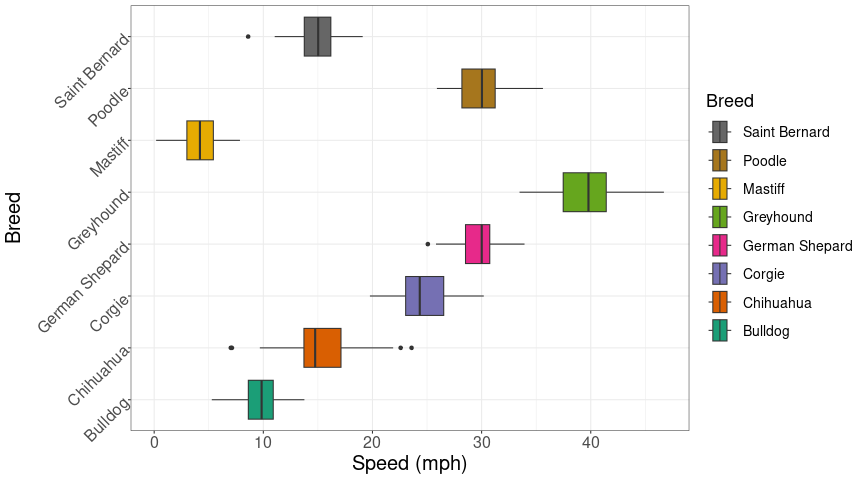
\includegraphics[scale=0.4]{img/dog_breed.png}
\end{center}

\end{frame}


\begin{frame}{The General Idea}
\large
The total variability of a sample can be broken into two parts:

\begin{itemize}
\item Variability within each group
\item Variability between groups
    \begin{itemize}
        \item how different are the group means/medians
    \end{itemize}
\end{itemize}
\vp \vspace{6mm}

How did variability \textit{between groups} and \textit{within groups} compare when we looked at dogs grouped by size versus by color or by breed?

\end{frame}

\begin{frame}{Types of Variability}

A common metric for describing variability is the 'sum of squares' giving total squared distance between observations and the overall mean \vspace{-2mm}

\begin{align*}
\text{SS}_{\text{total}} = \text{SST} = \sum_{\text{all } i,j} (x_{ij} - \overline{x})^2
\end{align*}

where $i = 1, \dots, k$ indicates the group and $j = 1, \dots, n$ indicates the observations within the group. \vspace{4mm}

We can always decompose this into two other sums of squares \vspace{-2mm}

\begin{align*}
\underbrace{\sum_{} (x_{ij} - \overline{x})^2}_{\substack{\text{Total} \\ \text{variability}}} = \underbrace{\sum_{j=1}^n (x_{ij} - \overline{x}_j)^2}_{\substack{\text{Variability} \\ \text{within groups}}} + \underbrace{\sum_{i=1}^k n_i(\overline{x}_i - \overline{x})^2}_{\substack{\text{Variability} \\ \text{between groups}}} 
\end{align*}

\end{frame}

\begin{frame}{Types of Variability}
\small
\begin{align*}
\underbrace{\sum_{} (x_{ij} - \overline{x})^2}_{\substack{\text{Total} \\ \text{variability}}} = \underbrace{\sum_{j=1}^n (x_{ij} - \overline{x}_j)^2}_{\substack{\text{Variability} \\ \text{within groups}}} + \underbrace{\sum_{i=1}^k n_i(\overline{x}_i - \overline{x})^2}_{\substack{\text{Variability} \\ \text{between groups}}} 
\end{align*}

\begin{center}
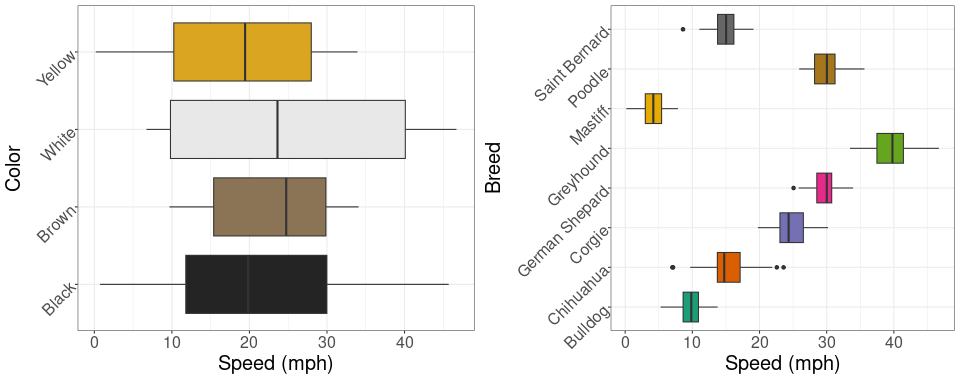
\includegraphics[scale=0.35]{img/dog_var_compare.png}
\end{center}

\end{frame}



\begin{frame}{Types of Variability}
Recall our null hypothesis for ANOVA

\begin{align*}
H_0&: \mu_1 = \mu_2 = \dots = \mu_k \\
H_A&: \text{at least one } \mu_i \not= \mu_j
\end{align*} \vspace{4mm}

\begin{itemize}
\item Low within group variabilty $\Leftrightarrow$ tight knit clearly defined group around a mean
\item High between group variability $\Leftrightarrow$ the groups are clearly distinct from one another
\end{itemize}
\end{frame}


\begin{frame}{Within-group Variability}
This measures how much variability there is within each group \vspace{6mm}

The summation corresponding to within-group variability is given a special name: \textit{sum of squared errors (SSE)} or $\text{SS}_{\text{error}}$
\begin{align*}
\text{SSE} = \sum_{j=1}^k (x_{ij} - \overline{x}_i)^2
\end{align*} \vspace{2mm}

This can also be written as the \textit{weighted} sum of group standard deviations
\begin{align*}
\text{SSE} = \sum_{i=1}^k (n_i- 1)s_i^2 = (n_1 - 1)s_1^2 + (n_2 - 1)s_2^2 + \dots + (n_k-1)s_k^2
\end{align*} \vspace{4mm}

\textbf{Intuition}: SSE is finding how far each observation is from it's group mean
\end{frame}

\begin{frame}{Variability between groups}
This describes how different each of the groups are from one another \vspace{10mm}

Also known as the sum of squares between groups (SSG), we can compute it by finding the weighted mean of group deviations:
\begin{align*}
SSG &= \sum n_i(\overline{x}_i - \overline{x})^2 \\
&= n_1(\overline{x}_1 - \overline{x})^2 + n_2(\overline{x}_2 - \overline{x})^2 + \dots + n_k(\overline{x}_k - \overline{x})^2
\end{align*} \vspace{4mm}

\textbf{Intuition}: SSG is finding how different each group mean is from the overall mean (and adjusting for \# of observations within that group)

\end{frame}

\begin{frame}{Degrees of Freedom}
When we calculated test-statistics before, we had a degree of freedom corresponding to how much information we used to estimate things

\begin{align*}
\text{SSE} = \sum_{j=1}^n (x_{ij} - \overline{x}_i)^2, \text{ for each of group i = 1,..., k}
\end{align*} \vspace{-2mm}

\begin{itemize}
    \item using $k$ group means, each has 50 observations $\rightarrow$ $n-k$ df
\end{itemize} \vspace{4mm}

\begin{align*}
SSG &= \sum n_i(\overline{x}_i - \overline{x})^2 \\
&= n_1(\overline{x}_1 - \overline{x})^2 + n_2(\overline{x}_2 - \overline{x})^2 + \dots + n_k(\overline{x}_k - \overline{x})^2
\end{align*}

\begin{itemize}
    \item using $k$ groups to estimate this $\rightarrow$ df = $k-1$
\end{itemize}

\end{frame}

\begin{frame}{Degrees of Freedom}
Frequently instead of using SSE and SSG directly, we will divide them by their respective degrees of freedom \vspace{10mm}

\textbf{Mean-Square-Error (Mean Square of Errors)}:
\begin{align*}
\text{MSE} = \frac{\text{SSE}}{n-k}
\end{align*} \vspace{4mm}

\textbf{Mean-Square-Groups (Mean Square of Groups)}:
\begin{align*}
\text{MSG} = \frac{\text{SSG}}{k-1}
\end{align*} \vspace{3mm}

Dividing the Sums of Squares like this adjusts them to account for the number of observations and numbers of groups, and makes comparing them easier
\end{frame}


\begin{frame}{F-statistic}
Ultimately what we will use to determine the outcome of our test is the ratio of 'between group variations' and 'variation from error' 

\begin{align*}
F = \frac{MSG}{MSE} 
\end{align*} \vspace{4mm}

What makes the $F$ statistic large?
\begin{itemize}
\item big $MSG$
\item small $MSE$
\end{itemize}
\end{frame} 


\begin{frame}{F distribution}
Just as we are able to use to $t$-distribution in finding $p$-values for the difference of two means, we can use the $F$ distribution to find a $p$-value for assessing the null hypothesis for ANOVA \vspace{8mm}

Generally speaking, we are in good shape if:
\begin{itemize}
\item The distributions of the groups are roughly normal
\item The variances between the groups are roughly similar. Generally so long as the standard deviation of one group doesn't exceed twice that of another
\end{itemize} \vspace{8mm}

Similar to the $t$-distribution, the $F$ distribution is associated with degrees of freedom, in this case two different df's for each of MSG and MSE
\end{frame}

\begin{frame}{F distribution}
\begin{center}
\includegraphics[scale=0.45]{img/Fdist.png}
\end{center}
\end{frame}



%
%
%



%
%\begin{frame}{No Groups}
%\begin{center}
%\includegraphics[scale=0.45]{img/no_groups.png}
%\end{center}
%\end{frame}
%
%\begin{frame}{Yes Groups}
%\begin{center}
%\includegraphics[scale=0.45]{img/yes_groups.png}
%\end{center}
%\end{frame}


\begin{frame}{Formulas}
\footnotesize
\begin{align*}
\underbrace{\sum (x_{ij} - \overline{x})^2}_{\text{SST}} = \underbrace{\sum_{i=1}^k n_i(\overline{x}_i - \overline{x})^2}_{\text{SSG}} +\underbrace{\sum_{j=1}^n (x_{ij} - \overline{x}_j)^2}_{\text{SSE}}
\end{align*}

%Try and have these written on the board first
\begin{itemize}
\item SST = SSG + SSE
\item SSE = sum of squares \textit{within groups}
\item SSG = sum of squares \textit{between groups}
\item $MSG = \frac{SSG}{k-1}$
\item $MSE = \frac{SSE}{n-k}$
\item $F = \frac{MSG}{MSE}$
\end{itemize}

{\footnotesize
\begin{table}[ht]
\centering
\def\arraystretch{1.5}
\begin{tabular}{lccccc}
  \hline
Source & df & Sum Sq & Mean Sq & F value & Pr($>$F) / $p$-value \\ 
  \hline
Group        & k-1 & SSG & $MSG = \frac{SSG}{k-1}$ & $F = \frac{MSG}{MSE}$ & Upper tail \\ 
  Error   & n-k & SSE & $MSE = \frac{SSE}{n-k}$ &  &  \\ 
   \hline
 Total & n - 1 & SSTotal & & & \\ \hline
\end{tabular}
\end{table}
}
\end{frame}

\begin{frame}{Example}
\scriptsize
\begin{align*}
\underbrace{\sum (x_{ij} - \overline{x})^2}_{\text{SST}} = \underbrace{\sum_{i=1}^k n_i(\overline{x}_i - \overline{x})^2}_{\text{SSG}} +\underbrace{\sum_{j=1}^n (x_{ij} - \overline{x}_j)^2}_{\text{SSE}}
\end{align*}
\begin{center}
i=1,...k for groups, j = 1,...,n for individual observations within a group
\end{center}
\normalsize
\begin{align*}
H_0: \mu_A = \mu_B = \mu_C
\end{align*}
\vspace{-8mm}
\begin{align*}
A &= \{5,3,6,2,4\}, \quad \overline{x}_A = 4, \quad s_A^2 = 2.5 \\
B &= \{8, 4, 5, 7\}, \ \  \quad \overline{x}_B = 6, \quad s_B^2 = 3.33 \\
C &= \{6, 9, 7, 10\}, \ \quad \overline{x}_C = 8, \quad s_C^2 = 3.33 \\
\end{align*}
\vspace{-15mm}
\begin{align*}
\overline{x} = 5.84, \quad N = 13
\end{align*}

\end{frame}

\begin{frame}[fragile]{ANOVA in R}
We can perform ANOVA in R using the \texttt{aov()} function

\begin{center}
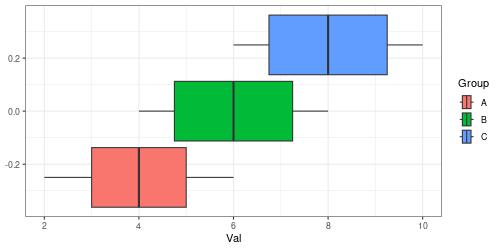
\includegraphics[scale=0.5]{example_group.png}
\end{center}

\begin{lstlisting}[language=R]
> aov(Val ~ Group, df) %>% summary()
            Df Sum Sq Mean Sq F value Pr(>F)  
Group        2   35.7    17.9    5.95   0.02 *
Residuals   10   30.0     3.0   
\end{lstlisting}

\end{frame}


\begin{frame}{Annual Temperature -- Grinnell}
\begin{center}
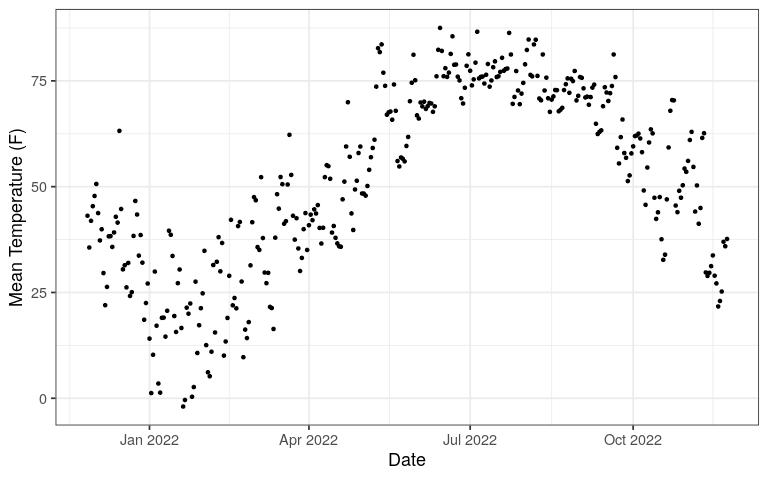
\includegraphics[scale=0.45]{img/just_temp.png}
\end{center}

\end{frame}

\begin{frame}{Annual Temperature}
\begin{center}
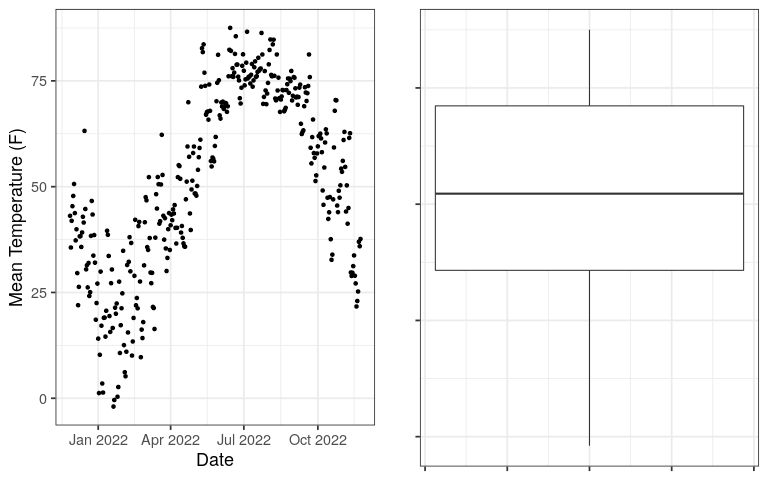
\includegraphics[scale=0.44]{img/tmp_and_bar.png}
\end{center}

\end{frame}

\begin{frame}{Temperature by Day}
\begin{center}
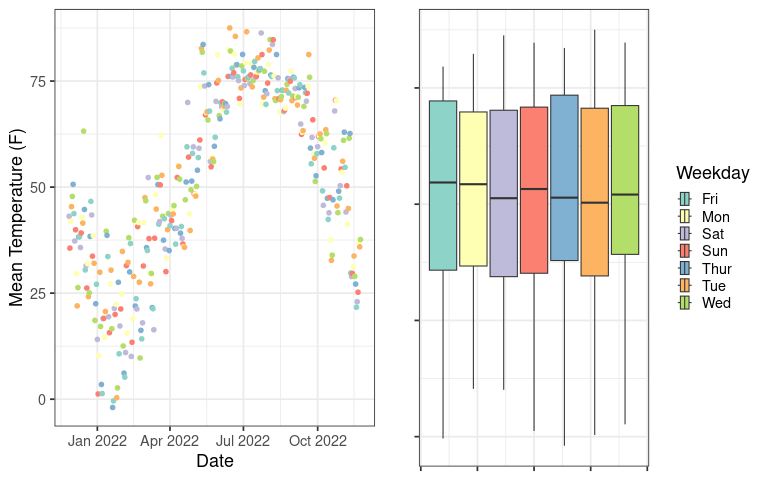
\includegraphics[scale=0.35]{img/tmp_weekday.png}
\end{center}
{\footnotesize
\begin{table}[ht]
\centering
\begin{tabular}{lrrrrr}
  \hline
 & Df & Sum Sq & Mean Sq & F value & Pr($>$F) \\ 
  \hline
Weekday     &  &  &  &  &  \\ 
  Residuals   &  &  &  &  &  \\ 
   \hline
\end{tabular}
\end{table}
}
\end{frame}

\begin{frame}{Temperature by Day}
\begin{center}
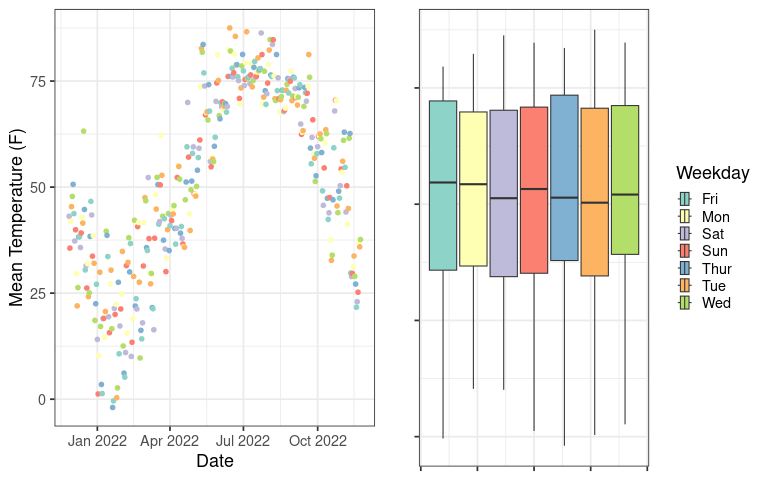
\includegraphics[scale=0.35]{img/tmp_weekday.png}
\end{center}
{\footnotesize
\begin{table}[ht]
\centering
\begin{tabular}{lrrrrr}
  \hline
 & Df & Sum Sq & Mean Sq & F value & Pr($>$F) \\ 
  \hline
Weekday     & 6 & 342.71 & 57.12 & 0.12 & 0.9939 \\ 
  Residuals   & 355 & 168524.83 & 474.72 &  &  \\ 
   \hline
\end{tabular}
\end{table}
}
\end{frame}

\begin{frame}{Temperature by Month}
\begin{center}
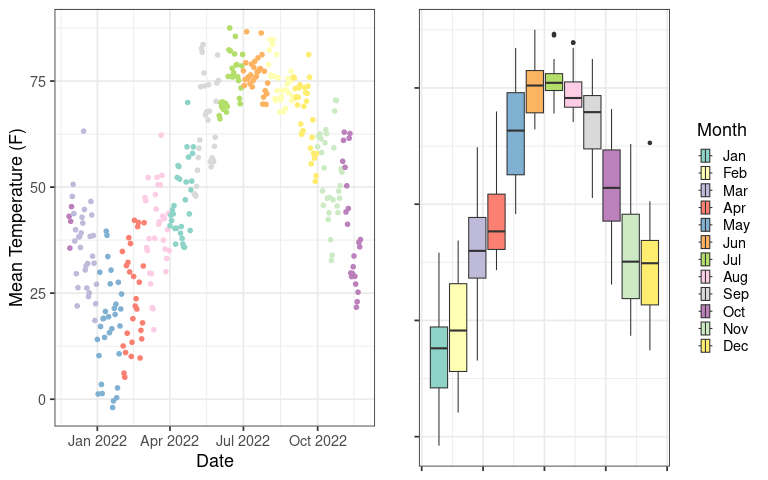
\includegraphics[scale=0.35]{img/tmp_month.png}
\end{center}
{\footnotesize
\begin{table}[ht]
\centering
\begin{tabular}{lrrrrr}
  \hline
 & Df & Sum Sq & Mean Sq & F value & Pr($>$F) \\ 
  \hline
Weekday     &  &  &  &  &  \\ 
  Residuals   &  &  &  &  &  \\ 
   \hline
\end{tabular}
\end{table}
}
\end{frame}

\begin{frame}{Temperature by Month}
\begin{center}
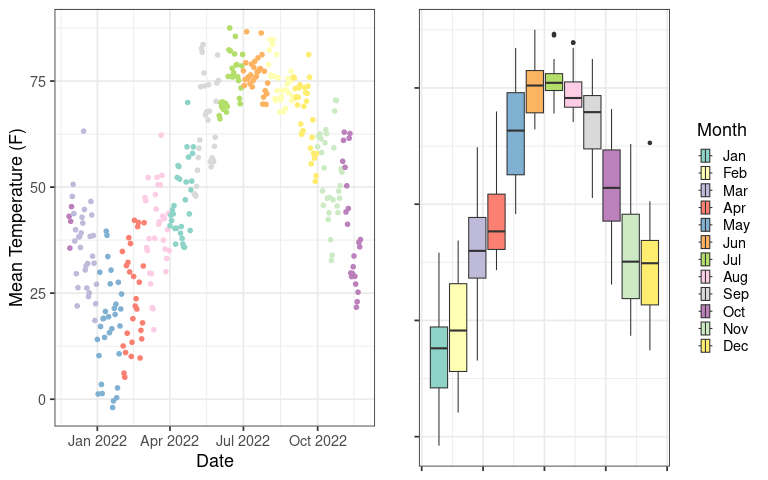
\includegraphics[scale=0.35]{img/tmp_month.png}
\end{center}
{\footnotesize
\begin{table}[ht]
\centering
\begin{tabular}{lrrrrr}
  \hline
 & Df & Sum Sq & Mean Sq & F value & Pr($>$F) \\ 
  \hline
Month       & 11 & 138048.06 & 12549.82 & 142.52 & $<$0.0001 \\ 
  Residuals   & 350 & 30819.48 & 88.06 &  &  \\ 
   \hline
\end{tabular}
\end{table}
}
\end{frame}


\begin{frame}{Review}

\textbf{ANOVA} is a method for finding out if group means are different
\begin{itemize}
    \item goal is to break down variability into different parts to help answer the question
\end{itemize} \vspace{6mm}

\begin{itemize}
\item Total variability made up of 'within' and 'between group' variation
\item F-statistic can be used to quantify how different these variabilities are from each other
\begin{itemize}
    \item F-distribution gives us our p-values
\end{itemize}
\end{itemize} \vspace{6mm}

Most of the time ANOVA info is arranged in a table so we can keep track of it
\end{frame}




\end{document}
